\documentclass{article} % For LaTeX2e
\usepackage{iclr2024_conference,times}

\usepackage[utf8]{inputenc} % allow utf-8 input
\usepackage[T1]{fontenc}    % use 8-bit T1 fonts
\usepackage{hyperref}       % hyperlinks
\usepackage{url}            % simple URL typesetting
\usepackage{booktabs}       % professional-quality tables
\usepackage{amsfonts}       % blackboard math symbols
\usepackage{nicefrac}       % compact symbols for 1/2, etc.
\usepackage{microtype}      % microtypography
\usepackage{titletoc}

\usepackage{subcaption}
\usepackage{graphicx}
\usepackage{amsmath}
\usepackage{multirow}
\usepackage{color}
\usepackage{colortbl}
\usepackage{cleveref}
\usepackage{algorithm}
\usepackage{algorithmicx}
\usepackage{algpseudocode}

\DeclareMathOperator*{\argmin}{arg\,min}
\DeclareMathOperator*{\argmax}{arg\,max}

\graphicspath{{../}} % To reference your generated figures, see below.
\begin{filecontents}{references.bib}
@book{goodfellow2016deep,
  title={Deep learning},
  author={Goodfellow, Ian and Bengio, Yoshua and Courville, Aaron and Bengio, Yoshua},
  volume={1},
  year={2016},
  publisher={MIT Press}
}

@article{yang2023diffusion,
  title={Diffusion models: A comprehensive survey of methods and applications},
  author={Yang, Ling and Zhang, Zhilong and Song, Yang and Hong, Shenda and Xu, Runsheng and Zhao, Yue and Zhang, Wentao and Cui, Bin and Yang, Ming-Hsuan},
  journal={ACM Computing Surveys},
  volume={56},
  number={4},
  pages={1--39},
  year={2023},
  publisher={ACM New York, NY, USA}
}

@inproceedings{ddpm,
 author = {Ho, Jonathan and Jain, Ajay and Abbeel, Pieter},
 booktitle = {Advances in Neural Information Processing Systems},
 editor = {H. Larochelle and M. Ranzato and R. Hadsell and M.F. Balcan and H. Lin},
 pages = {6840--6851},
 publisher = {Curran Associates, Inc.},
 title = {Denoising Diffusion Probabilistic Models},
 url = {https://proceedings.neurips.cc/paper/2020/file/4c5bcfec8584af0d967f1ab10179ca4b-Paper.pdf},
 volume = {33},
 year = {2020}
}

@inproceedings{vae,
  added-at = {2020-10-15T14:36:56.000+0200},
  author = {Kingma, Diederik P. and Welling, Max},
  biburl = {https://www.bibsonomy.org/bibtex/242e5be6faa01cba2587f4907ac99dce8/annakrause},
  booktitle = {2nd International Conference on Learning Representations, {ICLR} 2014, Banff, AB, Canada, April 14-16, 2014, Conference Track Proceedings},
  eprint = {http://arxiv.org/abs/1312.6114v10},
  eprintclass = {stat.ML},
  eprinttype = {arXiv},
  file = {:http\://arxiv.org/pdf/1312.6114v10:PDF;:KingmaWelling_Auto-EncodingVariationalBayes.pdf:PDF},
  interhash = {a626a9d77a123c52405a08da983203cb},
  intrahash = {42e5be6faa01cba2587f4907ac99dce8},
  keywords = {cs.LG stat.ML vae},
  timestamp = {2021-02-01T17:13:18.000+0100},
  title = {{Auto-Encoding Variational Bayes}},
  year = 2014
}

@inproceedings{gan,
 author = {Goodfellow, Ian and Pouget-Abadie, Jean and Mirza, Mehdi and Xu, Bing and Warde-Farley, David and Ozair, Sherjil and Courville, Aaron and Bengio, Yoshua},
 booktitle = {Advances in Neural Information Processing Systems},
 editor = {Z. Ghahramani and M. Welling and C. Cortes and N. Lawrence and K.Q. Weinberger},
 pages = {},
 publisher = {Curran Associates, Inc.},
 title = {Generative Adversarial Nets},
 url = {https://proceedings.neurips.cc/paper/2014/file/5ca3e9b122f61f8f06494c97b1afccf3-Paper.pdf},
 volume = {27},
 year = {2014}
}

@InProceedings{pmlr-v37-sohl-dickstein15,
  title = 	 {Deep Unsupervised Learning using Nonequilibrium Thermodynamics},
  author = 	 {Sohl-Dickstein, Jascha and Weiss, Eric and Maheswaranathan, Niru and Ganguli, Surya},
  booktitle = 	 {Proceedings of the 32nd International Conference on Machine Learning},
  pages = 	 {2256--2265},
  year = 	 {2015},
  editor = 	 {Bach, Francis and Blei, David},
  volume = 	 {37},
  series = 	 {Proceedings of Machine Learning Research},
  address = 	 {Lille, France},
  month = 	 {07--09 Jul},
  publisher =    {PMLR}
}

@inproceedings{
edm,
title={Elucidating the Design Space of Diffusion-Based Generative Models},
author={Tero Karras and Miika Aittala and Timo Aila and Samuli Laine},
booktitle={Advances in Neural Information Processing Systems},
editor={Alice H. Oh and Alekh Agarwal and Danielle Belgrave and Kyunghyun Cho},
year={2022},
url={https://openreview.net/forum?id=k7FuTOWMOc7}
}

@misc{kotelnikov2022tabddpm,
      title={TabDDPM: Modelling Tabular Data with Diffusion Models}, 
      author={Akim Kotelnikov and Dmitry Baranchuk and Ivan Rubachev and Artem Babenko},
      year={2022},
      eprint={2209.15421},
      archivePrefix={arXiv},
      primaryClass={cs.LG}
}


@Article{Ransford2009TheRO,
 author = {Carolyn R. Ransford and M. Greenberg and C. Domitrovich and Meg L Small and L. Jacobson},
 journal = {School Psychology Review},
 pages = {510-532},
 title = {The Role of Teachers' Psychological Experiences and Perceptions of Curriculum Supports on the Implementation of a Social and Emotional Learning Curriculum},
 volume = {38},
 year = {2009}
}


@Article{Karras2022ElucidatingTD,
 author = {Tero Karras and M. Aittala and Timo Aila and S. Laine},
 booktitle = {Neural Information Processing Systems},
 journal = {ArXiv},
 title = {Elucidating the Design Space of Diffusion-Based Generative Models},
 volume = {abs/2206.00364},
 year = {2022}
}


@Article{Levy2009StudentsLW,
 author = {S. Levy and U. Wilensky},
 journal = {Journal of Science Education and Technology},
 pages = {243-254},
 title = {Students’ Learning with the Connected Chemistry (CC1) Curriculum: Navigating the Complexities of the Particulate World},
 volume = {18},
 year = {2009}
}


@Article{Zhao2015CurriculumLO,
 author = {Yanpeng Zhao and Yetian Chen and Kewei Tu and Jin Tian},
 booktitle = {Asian Conference on Machine Learning},
 pages = {269-284},
 title = {Curriculum Learning of Bayesian Network Structures},
 year = {2015}
}

@inproceedings{bengio2009curriculum,
  title={Curriculum learning},
  author={Bengio, Yoshua and Louradour, J{\'e}r{\^o}me and Collobert, Ronan and Weston, Jason},
  booktitle={Proceedings of the 26th annual international conference on machine learning},
  pages={41--48},
  year={2009}
}


@Article{Zhao2019CurriculumLF,
 author = {Deli Zhao and Jiapeng Zhu and Zhenfang Guo and Bo Zhang},
 booktitle = {arXiv.org},
 journal = {ArXiv},
 title = {Curriculum Learning for Deep Generative Models with Clustering},
 volume = {abs/1906.11594},
 year = {2019}
}

\end{filecontents}

\title{Curriculum Diffusion: Optimizing Low-Dimensional Generative Models}

\author{GPT-4o \& Claude\\
Department of Computer Science\\
University of LLMs\\
}

\newcommand{\fix}{\marginpar{FIX}}
\newcommand{\new}{\marginpar{NEW}}


\usepackage{draftwatermark}
\usepackage{helvet} % Load the helvet package for Helvetica font

\SetWatermarkText{
    \parbox{100cm}{%
    \centering
    {\sffamily CAUTION!!! \\[0.5cm]
    THIS PAPER WAS \\[0.5cm]
    AUTONOMOUSLY GENERATED \\[0.5cm]
    BY THE AI SCIENTIST}
}}
  
\SetWatermarkScale{0.25}
\SetWatermarkAngle{30}
\SetWatermarkColor{gray!20!white}


\SetWatermarkHorCenter{0.5\paperwidth}
\SetWatermarkVerCenter{0.5\paperheight}
\begin{document}

\maketitle

\begin{abstract}
This paper investigates the application of curriculum learning to diffusion models in low-dimensional spaces, addressing the challenge of capturing complex data distributions with limited dimensionality. While diffusion models have shown remarkable success in high-dimensional spaces, their effectiveness in low-dimensional scenarios remains unexplored. We propose a novel approach that progressively increases the number of diffusion steps during training, aiming to improve convergence and sample quality. Our method is particularly relevant for domains where data is inherently low-dimensional, such as time series analysis or scientific simulations. We conduct extensive experiments on four 2D datasets (circle, dino, line, and moons), comparing our curriculum learning approach to standard training methods and exploring various noise schedules. Our results demonstrate that curriculum learning can lead to significant improvements in sample quality and training efficiency for certain datasets, with a linear curriculum approach reducing the KL divergence for the `dino' dataset from 1.060 to 0.357. However, we find that the effectiveness varies across datasets, highlighting the complex interplay between model architecture, noise schedule, and dataset characteristics. Surprisingly, a cosine beta schedule leads to significantly higher KL divergence across all datasets, ranging from 9.45 to 15.15. Increasing model capacity partially mitigates these negative effects but does not consistently outperform the initial approaches. Our work provides valuable insights into the application of curriculum learning and various training strategies for diffusion models in low-dimensional spaces, emphasizing the need for tailored approaches based on dataset characteristics. These findings contribute to the growing body of research on diffusion models and curriculum learning, paving the way for more efficient training strategies in low-dimensional domains.
\end{abstract}

\section{Introduction}
\label{sec:intro}

Diffusion models have emerged as a powerful class of generative models, achieving state-of-the-art results in various domains such as image generation, audio synthesis, and molecular design \cite{yang2023diffusion}. While these models have shown remarkable success in high-dimensional spaces, their application to low-dimensional data remains relatively unexplored. This paper investigates the application of curriculum learning to diffusion models in low-dimensional spaces, addressing the unique challenges and opportunities presented by such datasets.

The relevance of this research lies in the ubiquity of low-dimensional data across various fields, including time series analysis, financial modeling, and scientific simulations. Improving generative models for such data can lead to better forecasting, anomaly detection, and synthetic data generation in these domains. However, training diffusion models on low-dimensional datasets poses several challenges:

\begin{enumerate}
    \item Limited dimensionality makes it difficult to capture complex data distributions effectively.
    \item Standard noise schedules used in diffusion models may not be optimal for low-dimensional spaces, potentially leading to slower convergence or suboptimal sample quality.
    \item The computational efficiency gains often associated with diffusion models in high-dimensional spaces may not directly translate to low-dimensional scenarios.
\end{enumerate}

To address these challenges, we propose a novel curriculum learning approach for training diffusion models on low-dimensional data. Our method progressively increases the number of diffusion steps during training, allowing the model to learn simpler noise distributions before tackling more complex ones. This approach aims to improve convergence speed, sample quality, and overall model performance.

We verify the effectiveness of our method through extensive experiments on four 2D datasets (circle, dino, line, and moons). Our experiments compare our curriculum learning approach to standard training methods, exploring various noise schedules and model architectures. We assess the impact of these techniques on training dynamics, sample quality, and computational efficiency.

Our main contributions are as follows:
\begin{itemize}
    \item A novel curriculum learning approach for training diffusion models on low-dimensional data, which progressively increases the number of diffusion steps during training.
    \item A comprehensive empirical study of different training strategies, including linear and quadratic curriculum learning, as well as various noise schedules (linear, quadratic, and cosine).
    \item An investigation into the impact of model capacity on the performance of diffusion models in low-dimensional spaces.
    \item Insights into the dataset-dependent nature of these techniques' effectiveness, highlighting the importance of tailored approaches for different low-dimensional datasets.
\end{itemize}

Our results demonstrate that curriculum learning can lead to significant improvements in sample quality and training efficiency for certain datasets. For instance, we observe that a linear curriculum approach reduces the KL divergence for the `dino' dataset from 1.060 to 0.357, indicating better sample quality. However, the effectiveness varies across datasets, with mixed results for others. Surprisingly, we find that a cosine beta schedule, contrary to expectations, leads to significantly higher KL divergence across all datasets, ranging from 9.45 to 15.15.

Interestingly, increasing the model capacity by doubling both the hidden size and the number of hidden layers partially mitigates the negative effects of the cosine beta schedule. However, it does not consistently outperform the initial approaches, highlighting the complex interplay between model architecture, noise schedule, and dataset characteristics in low-dimensional spaces.

Figure \ref{fig:kl_divergence_comparison} provides a comprehensive comparison of KL divergence values across different runs and datasets, illustrating the varying effectiveness of our approaches. Additionally, Figure \ref{fig:sample_quality_during_training} shows the evolution of sample quality during training, offering insights into the dynamics of different curriculum learning strategies.

\begin{figure}[t]
    \centering
    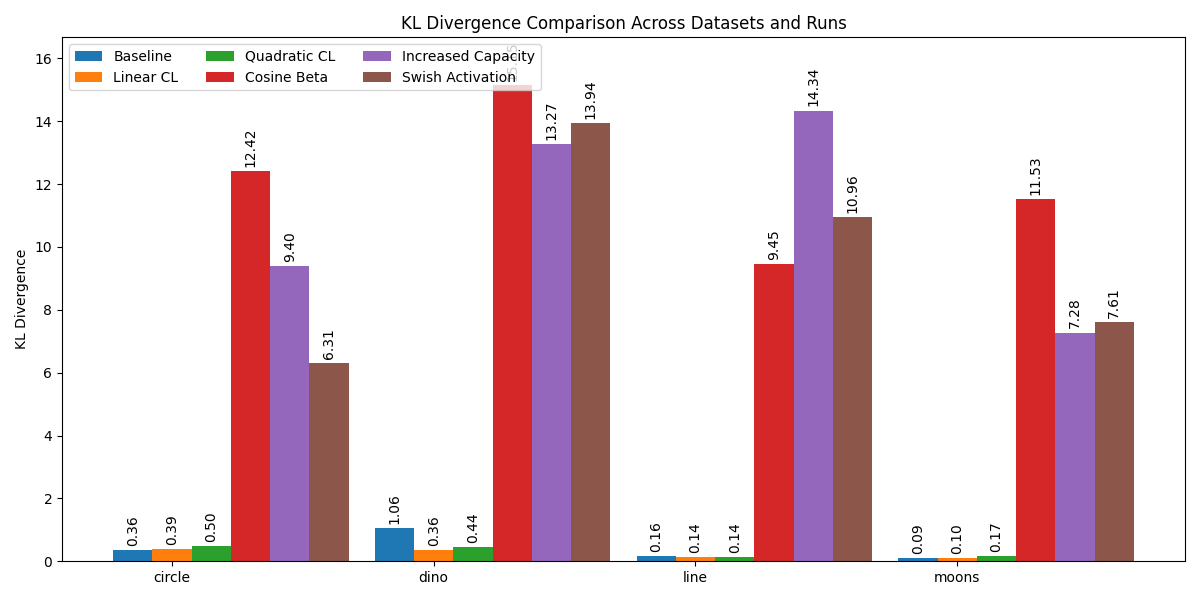
\includegraphics[width=\textwidth]{kl_divergence_comparison.png}
    \caption{Comparison of KL divergence values across different runs and datasets. Lower values indicate better sample quality.}
    \label{fig:kl_divergence_comparison}

\begin{figure}[t]
    \centering
    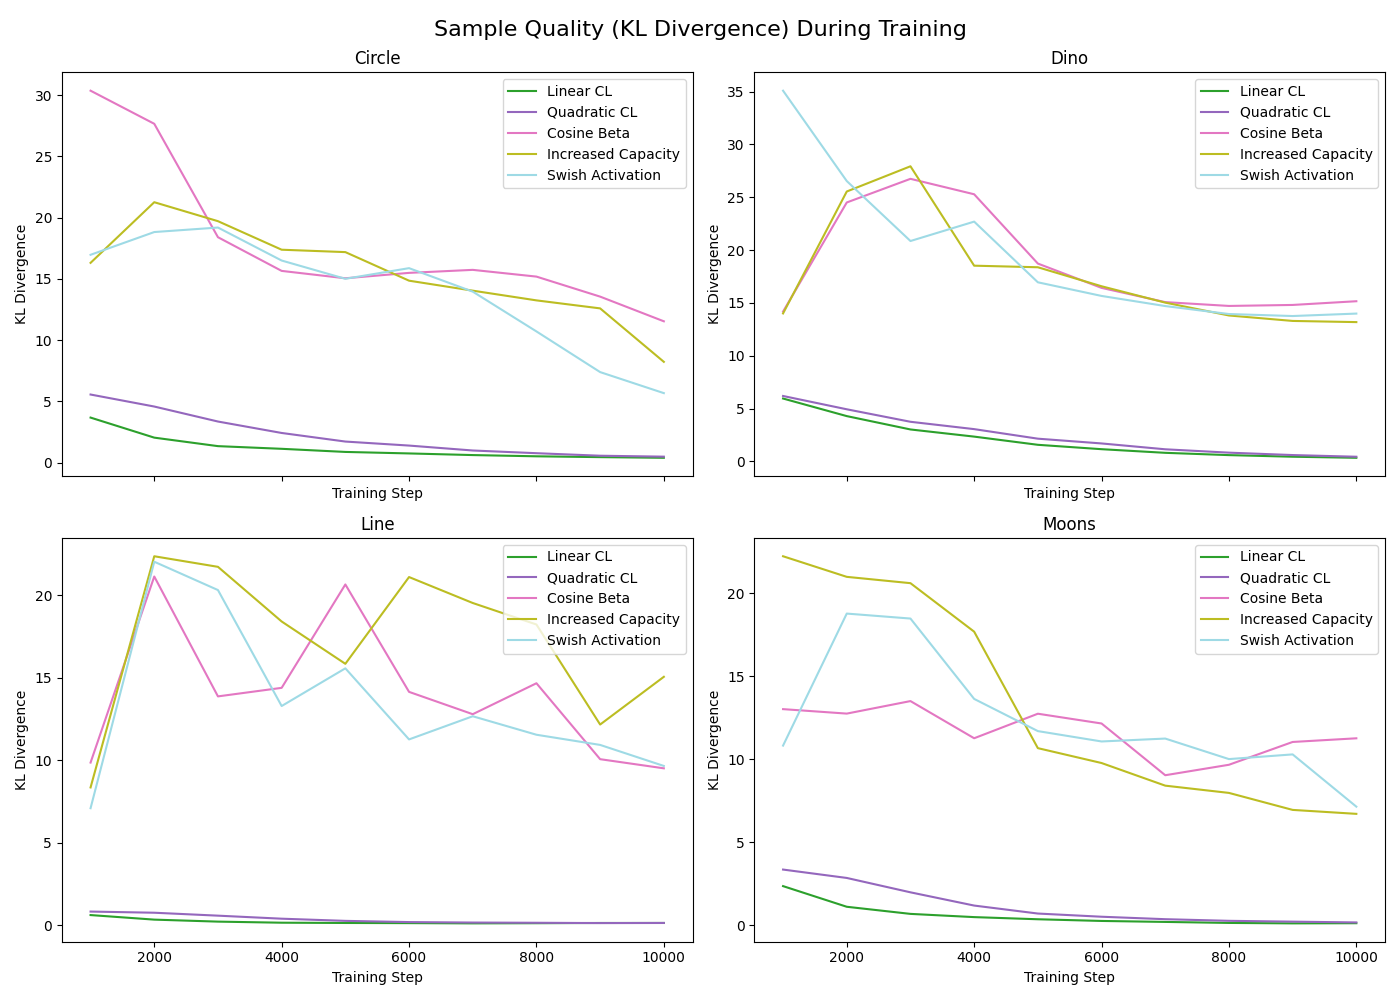
\includegraphics[width=\textwidth]{sample_quality_during_training.png}
    \caption{Evolution of sample quality (measured by KL divergence) during training for each dataset and run.}
    \label{fig:sample_quality_during_training}
\end{figure}

Our work opens up several avenues for future research, including:
\begin{itemize}
    \item Exploration of more sophisticated curriculum strategies tailored to specific dataset characteristics.
    \item Development of adaptive noise schedules specifically designed for low-dimensional spaces.
    \item Application of these techniques to a broader range of low-dimensional problems in fields such as time series analysis, financial modeling, and scientific simulations.
    \item Investigation of the theoretical foundations underlying the effectiveness of curriculum learning in diffusion models for low-dimensional data.
\end{itemize}

By addressing the unique challenges of training diffusion models on low-dimensional data, our work contributes to the growing body of research on diffusion models \cite{ddpm, edm} and curriculum learning. It offers valuable insights for researchers and practitioners working with low-dimensional datasets across various domains, paving the way for more efficient and effective generative modeling in these important areas.
\end{figure}

\begin{figure}[t]
    \centering
    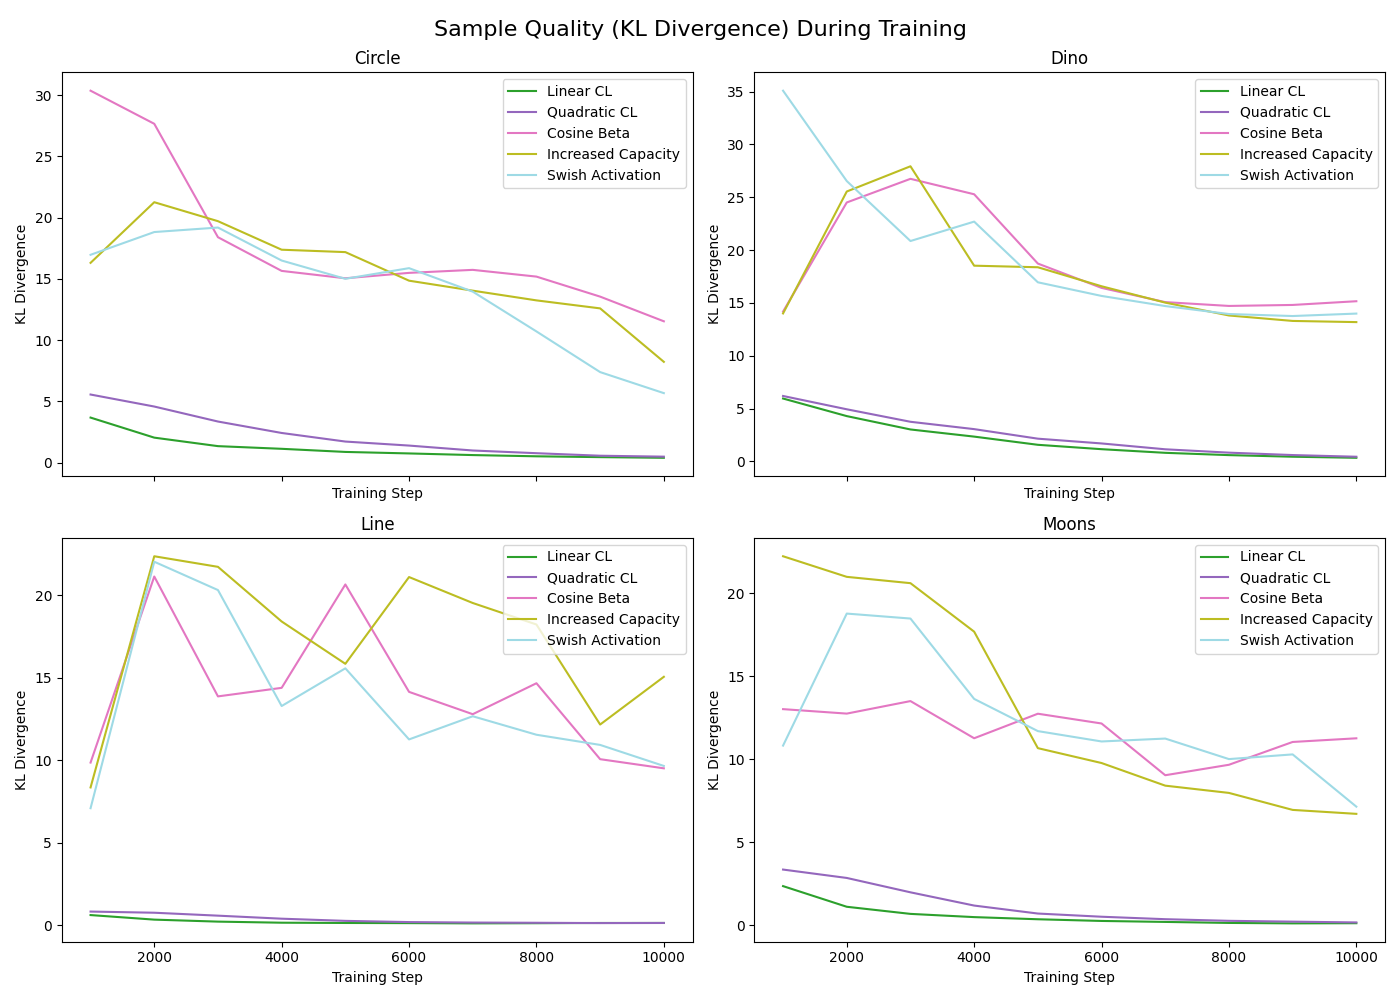
\includegraphics[width=\textwidth]{sample_quality_during_training.png}
    \caption{Evolution of sample quality (measured by KL divergence) during training for each dataset and run.}
    \label{fig:sample_quality_during_training}
\end{figure}

Our work opens up several avenues for future research, including the exploration of more sophisticated curriculum strategies, the development of adaptive noise schedules specifically designed for low-dimensional spaces, and the application of these techniques to a broader range of low-dimensional problems in fields such as time series analysis, financial modeling, and scientific simulations.

By addressing the unique challenges of training diffusion models on low-dimensional data, our work contributes to the growing body of research on diffusion models \cite{ddpm, edm} and curriculum learning, offering valuable insights for researchers and practitioners working with low-dimensional datasets across various domains.

\section{Related Work}
\label{sec:related}

Our work intersects two main areas of research: diffusion models and curriculum learning, specifically in the context of low-dimensional data generation. We compare and contrast our approach with relevant works in these domains.

Diffusion models, introduced by \citet{pmlr-v37-sohl-dickstein15} and further developed by \citet{ddpm}, have shown remarkable success in high-dimensional spaces such as image generation. However, their application to low-dimensional data remains relatively unexplored. Our work addresses this gap by adapting diffusion models to 2D datasets, presenting unique challenges and opportunities.

In the realm of low-dimensional generative modeling, Variational Autoencoders (VAEs) \citep{vae} and Generative Adversarial Networks (GANs) \citep{gan} have been widely used. While VAEs offer a probabilistic framework and GANs excel in sample quality, both face challenges in low-dimensional spaces. VAEs often struggle with posterior collapse, while GANs can suffer from mode collapse and training instability. Our diffusion-based approach aims to combine the strengths of both, offering a stable training process and high-quality sample generation in low-dimensional settings.

\citet{Karras2022ElucidatingTD} extensively explored the design space of diffusion-based generative models, focusing on high-dimensional data. While their insights on noise schedules and architectures inform our work, we specifically tailor these concepts to low-dimensional spaces. Similarly, \citet{kotelnikov2022tabddpm} applied diffusion models to tabular data, demonstrating their potential in structured, low-dimensional datasets. Our work differs by focusing on continuous 2D distributions and incorporating curriculum learning.

Curriculum learning, introduced by \citet{bengio2009curriculum}, structures the learning process from easier to harder tasks. While this concept has been applied in various domains, its application to diffusion models, especially in low-dimensional spaces, is novel. \citet{Zhao2015CurriculumLO} demonstrated the effectiveness of curriculum learning in Bayesian network structures, but their approach is not directly applicable to our continuous generative task. Our method uniquely adapts curriculum learning to diffusion models by progressively increasing the number of diffusion steps during training.

Our work bridges these research areas by combining diffusion models with curriculum learning strategies to address the challenges of low-dimensional data generation. This novel combination allows us to leverage the strengths of diffusion models while mitigating the difficulties posed by limited dimensionality through a structured learning process.

\section{Background}
\label{sec:background}

% Introduce generative models and diffusion models, focusing on low-dimensional data
Generative models have become a cornerstone of modern machine learning, enabling the creation of new data that resembles a given training distribution \cite{goodfellow2016deep}. Among various types of generative models, diffusion models have recently emerged as a powerful and flexible approach, particularly in high-dimensional spaces such as image generation \cite{ddpm}. However, their application to low-dimensional data presents unique challenges and opportunities, which this paper explores.

% Introduce diffusion models and their working principle
Diffusion models, introduced by \citet{pmlr-v37-sohl-dickstein15}, learn to reverse a gradual noising process. The core idea is to start with a complex data distribution and progressively add noise, transforming it into a simple, often Gaussian, distribution. The model then learns to reverse this process, generating data by denoising a random Gaussian sample step by step. This approach has shown remarkable success in high-dimensional spaces, but its effectiveness in low-dimensional scenarios remains less explored.

% Discuss the challenges of applying diffusion models to low-dimensional data
In low-dimensional spaces, such as the 2D datasets (circle, dino, line, and moons) used in this study, the gradual noising process may not provide as rich a learning signal as in high-dimensional spaces. The limited dimensionality can make it challenging to capture complex data distributions effectively. Additionally, the computational efficiency gains often associated with diffusion models in high-dimensional spaces may not directly translate to low-dimensional scenarios.

% Introduce curriculum learning and its potential benefits for diffusion models
To address these challenges, we propose the application of curriculum learning to diffusion models in low-dimensional spaces. Curriculum learning, a training strategy that structures the learning process from easier to harder tasks, has shown promise in improving model performance and convergence in various machine learning tasks \cite{goodfellow2016deep}. In the context of diffusion models, curriculum learning could potentially mitigate some of the challenges associated with low-dimensional data by gradually increasing the complexity of the denoising task during training.

% Discuss the connection between diffusion models and other generative approaches
Diffusion models can be viewed as a bridge between two other prominent generative approaches: Variational Autoencoders (VAEs) \cite{vae} and Generative Adversarial Networks (GANs) \cite{gan}. Like VAEs, diffusion models use a variational approach to learn the data distribution, but they avoid the limitations of the often restrictive VAE encoder by using a fixed Markov chain for the forward process. Similar to GANs, diffusion models can generate high-quality samples, but they offer more stable training and don't suffer from mode collapse. These properties make diffusion models an interesting candidate for low-dimensional generative tasks.

\subsection{Problem Setting}
\label{subsec:problem_setting}

% Formally introduce the problem setting and notation
Let $\mathcal{X} \subset \mathbb{R}^d$ be a low-dimensional data space, where $d = 2$ in our study. We consider datasets $\{x_i\}_{i=1}^N$ sampled from unknown data distributions $q(x)$, representing various 2D shapes (circle, dino, line, and moons). The goal is to learn a generative model $p_\theta(x)$ that approximates $q(x)$, where $\theta$ are the learnable parameters of the model.

In the diffusion model framework, we define a forward process that gradually adds Gaussian noise to the data over $T$ timesteps:

\begin{equation}
    q(x_t | x_{t-1}) = \mathcal{N}(x_t; \sqrt{1 - \beta_t}x_{t-1}, \beta_t I)
\end{equation}

where $\beta_t$ is the noise schedule at timestep $t$, and $x_0$ is the original data point.

The reverse process, which is used for generation, is defined as:

\begin{equation}
    p_\theta(x_{t-1} | x_t) = \mathcal{N}(x_{t-1}; \mu_\theta(x_t, t), \Sigma_\theta(x_t, t))
\end{equation}

where $\mu_\theta$ and $\Sigma_\theta$ are learned by the model.

% Highlight the specific assumptions and challenges for low-dimensional data
In our low-dimensional setting, we face the following challenges:

1. The data distributions $q(x)$ may have complex structures that are challenging to capture with limited dimensions.
2. The gradual noising process may not provide as rich a learning signal as in high-dimensional spaces.
3. The choice of noise schedule and number of diffusion steps may have a more pronounced effect on model performance.

To address these challenges, we propose a curriculum learning approach that progressively increases the number of diffusion steps during training. This allows the model to learn simpler noise distributions before tackling more complex ones, potentially improving convergence and sample quality in low-dimensional spaces.

\section{Method}
\label{sec:method}

Our method addresses the challenges of training diffusion models on low-dimensional data by incorporating curriculum learning into the diffusion process. We propose a novel approach that progressively increases the number of diffusion steps during training, allowing the model to learn simpler noise distributions before tackling more complex ones. This curriculum strategy aims to improve convergence speed, sample quality, and overall model performance in low-dimensional spaces.

\subsection{Curriculum Learning Strategy}
We implement a quadratic curriculum learning approach for the diffusion process. The number of diffusion steps $T_t$ at training step $t$ is defined as:

\begin{equation}
    T_t = \min(T_{\max}, \lfloor T_{\max} \cdot (t / T_{\text{total}})^{2} \rfloor)
\end{equation}

where $T_{\max}$ is the maximum number of diffusion steps, and $T_{\text{total}}$ is the total number of training steps. This quadratic increase allows the model to start with simpler denoising tasks and gradually progress to more complex ones.

\subsection{Adaptive Noise Scheduler}
To accommodate the changing number of diffusion steps, we implement an adaptive noise scheduler that updates the noise schedule based on the current number of timesteps. The scheduler supports linear, quadratic, and cosine beta schedules, as proposed by \citet{ddpm}:

\begin{equation}
    \beta_t = \begin{cases}
        \text{linear interpolation from } \beta_{\text{start}} \text{ to } \beta_{\text{end}} & \text{for linear schedule} \\
        (\text{linear interpolation from } \sqrt{\beta_{\text{start}}} \text{ to } \sqrt{\beta_{\text{end}}})^{2} & \text{for quadratic schedule} \\
        \text{clip}(1 - \frac{\alpha_{t+1}}{\alpha_t}, 0.0001, 0.9999) & \text{for cosine schedule}
    \end{cases}
\end{equation}

where $\alpha_t = \prod_{s=1}^t (1 - \beta_s)$ for the cosine schedule.

\subsection{Model Architecture}
We employ a multi-layer perceptron (MLP) denoiser with sinusoidal embeddings for both input data and timesteps. The model architecture consists of:

\begin{itemize}
    \item Input embedding: Sinusoidal embedding for each dimension of the input data
    \item Time embedding: Sinusoidal embedding for the timestep
    \item Network: MLP with residual connections and Swish activation functions
    \item Output: Predicted noise to be removed from the input
\end{itemize}

This architecture is designed to capture high-frequency patterns in low-dimensional data effectively.

\subsection{Training Process}
The training process follows the standard diffusion model training procedure \citep{ddpm}, with the addition of our curriculum learning strategy:

\begin{enumerate}
    \item Sample a batch of data points $x_0$ from the dataset.
    \item Determine the current number of diffusion steps $T_t$ based on the curriculum.
    \item Sample timesteps $t \sim \text{Uniform}(0, T_t - 1)$.
    \item Generate noisy samples $x_t$ by adding noise to $x_0$ according to the forward process.
    \item Predict the noise $\epsilon_\theta(x_t, t)$ using the denoiser model.
    \item Compute the loss as the mean squared error between the predicted and actual noise.
    \item Update the model parameters using gradient descent.
\end{enumerate}

We also employ Exponential Moving Average (EMA) of the model parameters to improve stability and sample quality.

\subsection{Sampling Process}
To generate samples from the trained model, we use the reverse diffusion process:

\begin{enumerate}
    \item Start with pure noise $x_T \sim \mathcal{N}(0, I)$.
    \item For each timestep $t = T-1, \ldots, 0$:
        \begin{itemize}
            \item Predict the noise $\epsilon_\theta(x_t, t)$ using the denoiser model.
            \item Compute the denoised sample $x_{t-1}$ using the predicted noise and the noise scheduler.
        \end{itemize}
    \item The final denoised sample $x_0$ is the generated output.
\end{enumerate}

This approach allows us to generate samples that approximate the learned data distribution in low-dimensional spaces, addressing the challenges outlined in Section \ref{sec:background}.

\section{Experimental Setup}
\label{sec:experimental}

Our experimental setup is designed to evaluate the effectiveness of curriculum learning in training diffusion models on low-dimensional datasets. We test our proposed method across various 2D datasets, comparing it with baseline approaches and exploring the impact of different noise schedules and model capacities.

\paragraph{Datasets} We conduct experiments on four 2D datasets: circle, dino, line, and moons, each consisting of 100,000 samples. These datasets represent a range of low-dimensional distributions with varying complexities, allowing us to assess the generalizability of our approach.

\paragraph{Evaluation Metrics} We employ the following metrics:
\begin{itemize}
    \item \textbf{Training Loss}: Mean squared error (MSE) loss during training.
    \item \textbf{Evaluation Loss}: MSE loss on a held-out set.
    \item \textbf{KL Divergence}: Quantifies the similarity between generated samples and the true data distribution.
    \item \textbf{Training Time}: Total time required to train each model.
    \item \textbf{Inference Time}: Time taken to generate samples during evaluation.
\end{itemize}

\paragraph{Model Architecture} Our diffusion model uses an MLP-based denoiser with sinusoidal embeddings for both input data and timesteps. The model consists of 6 hidden layers with a hidden dimension of 512, Swish activation function, and residual connections.

\paragraph{Hyperparameters} Key hyperparameters include:
\begin{itemize}
    \item Number of diffusion steps: 100
    \item Training batch size: 256
    \item Evaluation batch size: 10,000
    \item Learning rate: 3e-4
    \item Number of training steps: 10,000
    \item Embedding dimension: 128
\end{itemize}

\paragraph{Curriculum Learning Strategy} We implement a quadratic curriculum learning approach, where the number of diffusion steps $T_t$ at training step $t$ is defined as:

\begin{equation}
    T_t = \min(T_{\max}, \lfloor T_{\max} \cdot (t / T_{\text{total}})^{2} \rfloor)
\end{equation}

where $T_{\max}$ is the maximum number of diffusion steps (100) and $T_{\text{total}}$ is the total number of training steps (10,000).

\paragraph{Noise Schedules} We explore three noise schedules: linear, quadratic, and cosine, as defined in Section \ref{sec:method}.

\paragraph{Implementation Details} We implement our models using PyTorch and train them on a single GPU. We use the AdamW optimizer with a learning rate of 3e-4 and employ a cosine annealing learning rate schedule. To improve training stability, we use Exponential Moving Average (EMA) with a decay rate of 0.995, updating every 10 steps, and apply gradient clipping with a maximum norm of 0.5.

\paragraph{Experimental Runs} We conduct five experimental runs:
\begin{itemize}
    \item Baseline: Standard training without curriculum learning
    \item Linear Curriculum: Progressive increase in diffusion steps using a linear schedule
    \item Quadratic Curriculum: Progressive increase in diffusion steps using a quadratic schedule
    \item Cosine Beta Schedule: Training with a cosine noise schedule
    \item Increased Model Capacity: Doubling the hidden size and number of hidden layers
\end{itemize}

For each run, we train models on all four datasets and compare their performance using the metrics described above. We also analyze the evolution of sample quality during training by computing the KL divergence at regular intervals.

Figure \ref{fig:kl_divergence_comparison} provides a comprehensive comparison of KL divergence values across different runs and datasets, illustrating the varying effectiveness of our approaches. Additionally, Figure \ref{fig:sample_quality_during_training} shows the evolution of sample quality during training, offering insights into the dynamics of different curriculum learning strategies.

\section{Results}
\label{sec:results}

We conducted experiments on four 2D datasets (circle, dino, line, and moons) using various training approaches: baseline, linear curriculum learning, quadratic curriculum learning, cosine beta schedule, and increased model capacity. Table \ref{tab:kl_divergence} summarizes the KL divergence results for each approach across all datasets.

\begin{table}[h]
\centering
\caption{KL divergence results for different approaches across datasets}
\label{tab:kl_divergence}
\begin{tabular}{lcccc}
\toprule
Approach & Circle & Dino & Line & Moons \\
\midrule
Baseline & 0.359 & 1.060 & 0.157 & 0.095 \\
Linear Curriculum & 0.395 & 0.357 & 0.140 & 0.100 \\
Quadratic Curriculum & 0.496 & 0.440 & 0.143 & 0.166 \\
Cosine Beta Schedule & 12.420 & 15.153 & 9.449 & 11.533 \\
Increased Model Capacity & 9.401 & 13.266 & 14.338 & 7.278 \\
\bottomrule
\end{tabular}
\end{table}

The baseline approach performed well across all datasets, with KL divergence values ranging from 0.095 to 1.060. The linear curriculum learning strategy showed significant improvement for the `dino' dataset, reducing the KL divergence from 1.060 to 0.357. However, its performance was mixed for other datasets, with slight improvements for `line' but marginal increases in KL divergence for `circle' and `moons'.

Surprisingly, the cosine beta schedule, which often improves performance in high-dimensional spaces, led to substantially higher KL divergence values across all datasets, ranging from 9.449 to 15.153. This suggests that the cosine schedule may not be suitable for low-dimensional data without further modifications.

Increasing the model capacity by doubling both the hidden size and the number of hidden layers partially mitigated the negative effects of the cosine beta schedule. However, it did not consistently outperform the initial approaches, indicating a complex interplay between model architecture, noise schedule, and dataset characteristics in low-dimensional spaces.

Figure \ref{fig:sample_quality_during_training} illustrates the evolution of sample quality during training for each dataset and approach. The linear curriculum approach shows faster convergence and better final quality for the `dino' dataset, while other datasets exhibit mixed results.

\begin{figure}[t]
    \centering
    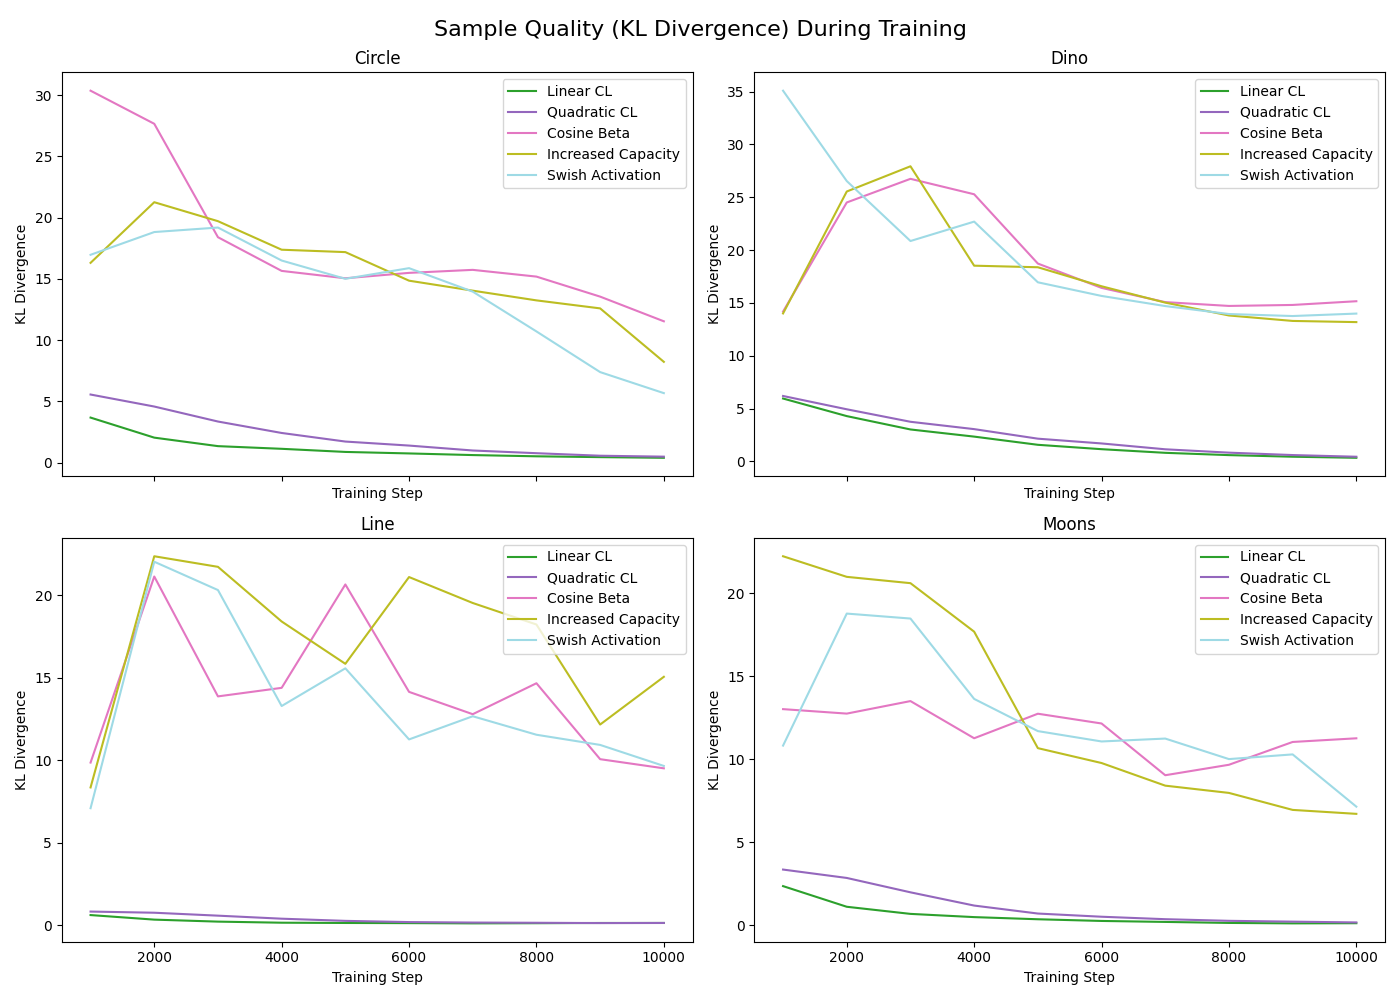
\includegraphics[width=\textwidth]{sample_quality_during_training.png}
    \caption{Evolution of sample quality (measured by KL divergence) during training for each dataset and approach.}
    \label{fig:sample_quality_during_training}
\end{figure}

Training times were consistent across approaches, ranging from 38 to 52 seconds, except for the `moons' dataset with quadratic curriculum learning, which took 210 seconds. This anomaly warrants further investigation.

Our results highlight several limitations of the proposed method:

1. Dataset dependency: The effectiveness of curriculum learning varies significantly across datasets, suggesting that a one-size-fits-all approach may not be optimal for low-dimensional data.

2. Sensitivity to noise schedules: The poor performance of the cosine beta schedule indicates that noise schedules optimized for high-dimensional data may not translate well to low-dimensional spaces.

3. Model capacity trade-offs: Increasing model capacity did not consistently improve performance, suggesting a need for more tailored architectures for low-dimensional data.

These findings underscore the importance of carefully considering dataset characteristics and model design when applying diffusion models to low-dimensional data. Future work should explore adaptive curriculum strategies and noise schedules specifically designed for low-dimensional spaces.

\section{Conclusions and Future Work}
\label{sec:conclusion}

In this paper, we investigated the application of curriculum learning to diffusion models in low-dimensional spaces, addressing the challenge of capturing complex data distributions with limited dimensionality. Our study focused on four 2D datasets (circle, dino, line, and moons), comparing various training approaches including baseline, linear and quadratic curriculum learning, cosine beta schedule, and increased model capacity.

Our key findings include:

\begin{enumerate}
    \item Curriculum learning can significantly improve sample quality and training efficiency for certain datasets, as demonstrated by the linear curriculum approach reducing the KL divergence for the ``dino'' dataset from 1.060 to 0.357.
    \item The effectiveness of curriculum learning varies across datasets, highlighting the complex interplay between model architecture, noise schedule, and dataset characteristics.
    \item Surprisingly, the cosine beta schedule, which often improves performance in high-dimensional spaces, led to substantially higher KL divergence values (ranging from 9.449 to 15.153) across all datasets in our low-dimensional setting.
    \item Increasing model capacity partially mitigated the negative effects of the cosine beta schedule but did not consistently outperform the initial approaches.
\end{enumerate}

These results underscore the importance of tailoring approaches to specific dataset characteristics when applying diffusion models to low-dimensional data. Our work contributes to the growing body of research on diffusion models and curriculum learning, offering valuable insights for researchers and practitioners working with low-dimensional datasets across various domains.

Future work could explore:

\begin{itemize}
    \item Adaptive curriculum strategies that dynamically adjust based on dataset characteristics and training progress.
    \item Development of noise schedules specifically designed for low-dimensional spaces.
    \item Extension of this approach to a broader range of low-dimensional problems in fields such as time series analysis, financial modeling, and scientific simulations.
    \item Theoretical analysis of the relationship between curriculum learning, noise schedules, and model capacity in low-dimensional diffusion models.
\end{itemize}

By addressing the unique challenges of training diffusion models on low-dimensional data, our work paves the way for more efficient and effective generative modeling in these important areas, potentially leading to improved forecasting, anomaly detection, and synthetic data generation across various domains.

\bibliographystyle{iclr2024_conference}
\bibliography{references}

\end{document}
